% Ch. 3, Fig. 3.2: which entries of the evaluation matrix each continual-learning metric uses.
% Definitions: thesis/background.tex Sec. 3.4, scripts/compute_cl_metrics.py. Build: python scripts/build_tikz.py
%
% PLAN
% Five panels (2026-10-22: Average Performance dropped): row 1 P1 P2 P3 (primary metrics),
% row 2 P4 P5 (secondary), P4 centred under the midpoint of P1 and P2. Each a T x (T+1) matrix (T = 6):
%   rows = task i = 1..T (top to bottom), columns = stage j = 0..T (left to right), plus one
%   control row c_j below the matrix (gap 1.5 mm). Cell (i, j) = node Pk-i-(j+1); control cell = Pkc-1-(j+1).
% Placement: P1 at the origin; P2 right=17mm of P1, P3 right=17mm of P2 (room for the left labels);
%   P4 below=19mm of the midpoint of P1c and P2c (room for title and column labels), P5 right of P4.
% Labels per panel (same offsets in every panel): column ticks "0", "T" above cells (1,1), (1,7),
%   "stage j" above cell (1,4); title above that; row ticks "1", "T", "c" left of (1,1), (6,1), control;
%   "task i" rotated, left of the rows. Legend centred below row 2: two swatches.
% Marks: hl (dark) = entries averaged in the metric; ref (light) = entries the metric subtracts from
%   (maximum over earlier stages, pretrained value).
% No connections (no arrows) in this figure.
\documentclass[12pt,tikz,border=2pt]{standalone}
% Shared preamble of the standalone TikZ figures: same engine, class size, fonts and
% math packages as thesis_main.tex (pdfLaTeX, 12 pt, T1 + Latin Modern, amsmath, bm).
\usepackage[utf8]{inputenc}
\usepackage[T1]{fontenc}
\usepackage{lmodern}
\usepackage{amsmath,amssymb,bm}
\usepackage{graphicx}
\usepackage{xcolor}
\usetikzlibrary{arrows.meta, positioning, calc, fit, backgrounds, decorations.pathreplacing}
\pgfdeclarelayer{panel}            % below the background layer: large panel frames
\pgfsetlayers{panel,background,main}
\def\mat#1{\ensuremath{\bm#1}}   % as lmedoc/math.sty
\def\vec#1{\ensuremath{\bm#1}}
% Colours: base colours of the VoxTell sketch, one colour per strategy component
\definecolor{voxorange}{HTML}{F2A65A}
\definecolor{voxblue}{HTML}{6CA6E0}
\definecolor{voxgreen}{HTML}{8DBF8B}
\definecolor{voxyellow}{HTML}{F5D76E}
\definecolor{voxred}{HTML}{E8877F}
\definecolor{voxlora}{HTML}{D1495B}
\definecolor{voxprompt}{HTML}{7A4FC9}
\definecolor{voxmeta}{HTML}{1B8A8F}
\definecolor{voxkd}{HTML}{C2308F}
\tikzset{lock/.pic={
  \draw[line width=0.6pt] (-0.07,0.02) -- (-0.07,0.09) arc[start angle=180, end angle=0, radius=0.07] -- (0.07,0.02);
  \fill[black!70] (-0.1,-0.1) rectangle (0.1,0.03);
}}
\newif\ifvoximpl     % VoxTell as used (stage-4 keys/values) instead of as in the paper (bottleneck)
\newif\ifvoxannotate
\newif\ifvoxpanel

\usetikzlibrary{matrix}
\begin{document}
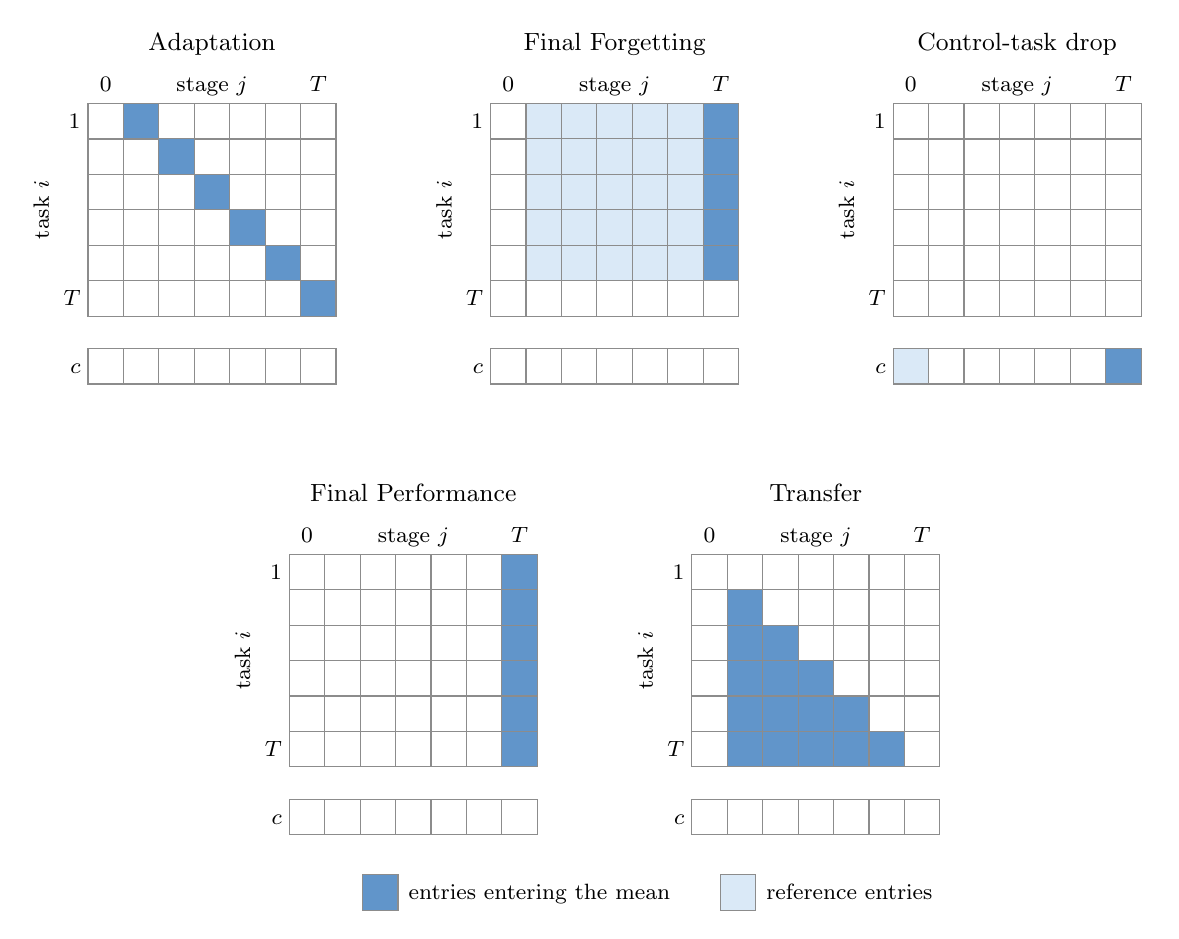
\begin{tikzpicture}[
    font=\small,
    cell/.style={draw=black!45, line width=0.4pt, minimum size=4.5mm, inner sep=0pt, outer sep=0pt},
    hl/.style={fill=voxblue!90!black},
    ref/.style={fill=voxblue!25},
    tick/.style={font=\footnotesize, inner sep=0.8pt, text height=1.6ex, text depth=0.4ex},
    ttl/.style={font=\small, inner sep=1pt, text height=1.7ex, text depth=0.5ex},
  ]
\def\pgap{17mm}
% \panel{name}{title}{placement}
\newcommand{\panel}[3]{%
  \matrix (#1) [matrix of nodes, nodes in empty cells, nodes={cell},
                column sep=-0.4pt, row sep=-0.4pt, ampersand replacement=\&, #3] {
    \&\&\&\&\&\&\\ \&\&\&\&\&\&\\ \&\&\&\&\&\&\\ \&\&\&\&\&\&\\ \&\&\&\&\&\&\\ \&\&\&\&\&\&\\ };
  \matrix (#1c) [matrix of nodes, nodes in empty cells, nodes={cell},
                 column sep=-0.4pt, ampersand replacement=\&, below=1.5mm of #1] { \&\&\&\&\&\&\\ };
  \node[tick, anchor=south] (#1t0) at ([yshift=0.6mm]#1-1-1.north) {$0$};
  \node[tick, anchor=south] (#1tT) at ([yshift=0.6mm]#1-1-7.north) {$T$};
  \node[tick, anchor=south] (#1tj) at ([yshift=0.6mm]#1-1-4.north) {stage $j$};
  \node[ttl, anchor=south] at ([yshift=1.2mm]#1tj.north) {#2};
  \node[tick, anchor=east] at ([xshift=-0.6mm]#1-1-1.west) {$1$};
  \node[tick, anchor=east] at ([xshift=-0.6mm]#1-6-1.west) {$T$};
  \node[tick, anchor=east] at ([xshift=-0.6mm]#1c-1-1.west) {$c$};
  \node[tick, rotate=90, anchor=south] at ([xshift=-4mm]#1-3-1.south west) {task $i$};
}
% \mark{style}{matrix}{row}{column}: shade one cell without moving its border
\newcommand{\mk}[4]{\fill[#1] (#2-#3-#4.north west) rectangle (#2-#3-#4.south east);
                    \draw[draw=black!45, line width=0.4pt] (#2-#3-#4.north west) rectangle (#2-#3-#4.south east);}

% Row 1: primary metrics; row 2: secondary metrics, centred under the gaps of row 1.
\panel{P1}{Adaptation}{}
\panel{P2}{Final Forgetting}{right=\pgap of P1}
\panel{P3}{Control-task drop}{right=\pgap of P2}
\coordinate (r2) at ($(P1c.south)!0.5!(P2c.south)$);
\panel{P4}{Final Performance}{below=19mm of r2}
\panel{P5}{Transfer}{right=\pgap of P4}

% Adaptation: diagonal a_{i,i}
\foreach \i in {1,...,6} { \pgfmathtruncatemacro{\c}{\i+1} \mk{hl}{P1}{\i}{\c} }
% Final Forgetting: i = 1..T-1; max over j = 1..T-1 (ref), final a_{i,T} (hl)
\foreach \i in {1,...,5} { \foreach \c in {2,...,6} { \mk{ref}{P2}{\i}{\c} } \mk{hl}{P2}{\i}{7} }
% Control-task drop: c_0 (ref) minus c_T (hl)
\mk{ref}{P3c}{1}{1} \mk{hl}{P3c}{1}{7}
% Final Performance: a_{i,T}
\foreach \i in {1,...,6} { \mk{hl}{P4}{\i}{7} }
% Transfer: a_{i,j}, 1 <= j < i
\foreach \i in {2,...,6} { \pgfmathtruncatemacro{\last}{\i} \foreach \c in {2,...,\last} { \mk{hl}{P5}{\i}{\c} } }

% Legend centred below the second row
\coordinate (lgc) at ($(P4c.south)!0.5!(P5c.south) + (0,-6mm)$);
\node[cell, hl, anchor=west] (lg1) at ([xshift=-32mm]lgc) {};
\node[tick, right=1mm of lg1] (lt1) {entries entering the mean};
\node[cell, ref, right=6mm of lt1] (lg2) {};
\node[tick, right=1mm of lg2] {reference entries};
\end{tikzpicture}
\end{document}
